\section{Umweltkatastrophe und Umweltbewusstsein}

\subsection{Einführung: Umwelt als technikgeschichtliches Problem}

Die Vorlesung untersucht,
wie Umweltkatastrophen und Umweltbewusstsein
im Verlauf des 20. Jahrhunderts
zu zentralen Themen moderner Technikgeschichte wurden.

Im Zentrum steht die Frage,
wie technische,
industrielle und wirtschaftliche Entwicklungen
neue Risiken hervorbrachten
und wie diese Risiken gesellschaftlich,
politisch und wissenschaftlich wahrgenommen wurden.

Umweltprobleme erscheinen dabei nicht nur
als Folgen einzelner Unfälle.

Sie entstehen auch durch langfristige,
schleichende Prozesse,
die mit moderner Produktion,
Konsum,
Energieversorgung
und globalen Stoffkreisläufen verbunden sind.

Zentrale Leitfragen:

\begin{itemize}
\item Wie entstehen technische Umweltkatastrophen?
\item Was unterscheidet plötzliche Katastrophen von schleichenden Krisen?
\item Warum wird Umwelt erst im 20. Jahrhundert zu einem gesellschaftspolitischen Problem?
\item Welche Rolle spielen Wissenschaft, Medien und Protestbewegungen?
\item Welche politischen Antworten wurden auf Umweltprobleme entwickelt?
\end{itemize}

Die Geschichte des Umweltbewusstseins ist daher
nicht nur Naturgeschichte,
sondern auch Technik-,
Wissenschafts-,
Medien-,
Politik-
und Gesellschaftsgeschichte.

\subsection{Brandkatastrophe in Schweizerhalle 1986}

Ein zentrales Beispiel der Vorlesung
ist die Brandkatastrophe in Schweizerhalle.

In der Nacht vom 1. November 1986
brach in einer Lagerhalle des Chemiekonzerns Sandoz
bei Schweizerhalle nahe Muttenz
ein Grossbrand aus.

Bei den Löscharbeiten der Feuerwehr
gelangten tonnenweise Chemikalien in den Rhein.

Die Folgen waren massiv.

Der Rhein verfärbte sich zeitweise rot,
und bis weit flussabwärts kam es
zu starkem Fischsterben.

Besonders betroffen war die Aalpopulation.

Auf einer Länge von rund 400 Kilometern
starb die gesamte Aalpopulation
von etwa 150 000 Individuen.

Die Katastrophe machte sichtbar,
wie eng industrielle Produktion,
Flüsse,
Ökosysteme
und internationale Räume miteinander verbunden sind.

Ein lokaler Brand wurde dadurch
zu einem grenzüberschreitenden Umweltproblem.

\begin{center}
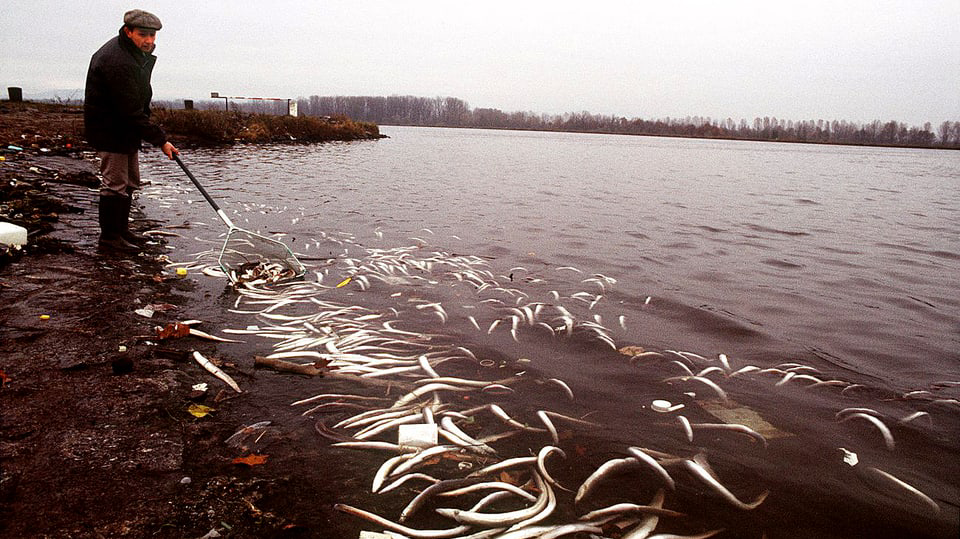
\includegraphics[width=0.8\linewidth]{images/schweizerhalle_brandkatastrophe.png}
\end{center}

\subsection{Quellenkritik zur Berichterstattung}

Die Vorlesung arbeitet am Beispiel
der Neuen Zürcher Zeitung vom 3. und 4. November 1986
auch quellenkritisch.

Untersucht werden soll,
wie über die Brandkatastrophe berichtet wurde
und welche Aspekte besonders hervorgehoben wurden.

Wichtige Fragen sind:

\begin{itemize}
\item Was berichten die Ausgaben vom 3. und 4. November?
\item Welche Aspekte der Katastrophe stehen im Vordergrund?
\item Wie unterscheiden sich die Beiträge der beiden Tage?
\item Warum wurde erst am 3. November berichtet, obwohl der Brand bereits am 1. November stattfand?
\item Welche Aspekte werden nicht erwähnt?
\end{itemize}

Diese Fragen zeigen,
dass Katastrophen nicht nur technische
oder ökologische Ereignisse sind.

Sie werden auch medial verarbeitet.

Was sichtbar wird,
welche Verantwortung benannt wird
und welche Fragen ausgeblendet bleiben,
ist Teil der gesellschaftlichen Auseinandersetzung
mit technischen Risiken.

\subsection{Ursachen und Verantwortung}

Bei Schweizerhalle stellte sich rasch
die Frage nach der Ursache des Brandes
und nach der Verantwortung.

Als mögliche Ursachen wurden
verschiedene Erklärungen diskutiert.

Dazu gehörten:

\begin{itemize}
\item Selbstentzündung durch chemische Reaktionen im Lager
\item unsachgemässe Lagerung verschiedener Produkte
\item menschliches Versagen
\item andere Zündquellen
\end{itemize}

Später wurde auch darüber berichtet,
dass möglicherweise Feuerwerkskörper
in der Halle gelagert gewesen seien.

Diese seien angeblich für die Verabschiedung
eines Kadermitarbeiters vorgesehen gewesen.

Die Frage nach der Ursache ist deshalb komplex.

Sie lässt sich nicht einfach
auf eine einzelne Person,
einen einzelnen Fehler
oder eine einzelne technische Störung reduzieren.

Vielmehr verweist sie
auf Lagerpraktiken,
Sicherheitskulturen,
Unternehmensorganisation,
chemische Prozesse
und technische Infrastrukturen.

\subsection{„Normale“ Umweltkatastrophen}

Die Brandkatastrophe von Schweizerhalle
steht in einer Reihe grosser Umwelt-
und Technikkatastrophen der 1970er und 1980er Jahre.

In den zehn Jahren vor Schweizerhalle
ereigneten sich unter anderem:

\begin{itemize}
\item 1976: Chemieunfall von Seveso in Italien
\item 1978: Öltankerunglück der Amoco Cadiz vor der Bretagne
\item 1979: Reaktorkatastrophe von Three Mile Island in den USA
\item 1984: Chemiekatastrophe von Bhopal in Indien
\item 1986: Reaktorkatastrophe von Tschernobyl in der Ukraine
\end{itemize}

Diese Ereignisse verstärkten den Eindruck,
dass moderne Grosstechnologien
nicht nur Fortschritt,
Wohlstand und Effizienz erzeugen,
sondern auch neue Formen systemischer Risiken.

Katastrophen erschienen nicht mehr
als seltene Ausnahmen,
sondern als mögliche Normalfolge
hochkomplexer technischer Systeme.

\begin{center}
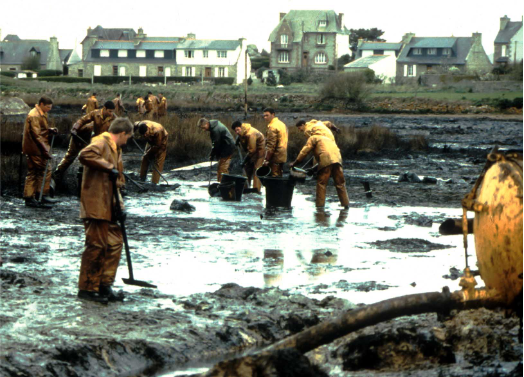
\includegraphics[width=0.75\linewidth]{images/normale_umweltkatastrophen.png}
\end{center}

\subsection{Charles Perrow und normale Katastrophen}

Der Soziologe Charles Perrow
prägte den Begriff der „normalen Katastrophen“.

Damit meinte er,
dass Katastrophen in komplexen
und eng gekoppelten technischen Systemen
nicht einfach vermeidbare Ausnahmen sind.

Moderne Grosstechnologien bestehen
aus vielen Teilsystemen,
die voneinander abhängig sind.

Wenn diese Systeme eng gekoppelt sind,
können kleine Störungen
schnell und unvorhersehbar
zu grösseren Krisen eskalieren.

Unfälle entstehen daher nicht nur
durch „menschliches Versagen“.

Sie entstehen aus dem Zusammenspiel
von Technik,
Organisation,
Kontrollsystemen,
Umweltbedingungen
und menschlichen Handlungen.

Sicherheitsmassnahmen können dabei
neue Komplexität erzeugen.

Zusätzliche Kontrollsysteme
schaffen manchmal neue Fehlerquellen.

Das bedeutet:

In komplexen technischen Systemen
können Katastrophen selbst dann entstehen,
wenn einzelne Beteiligte
nicht eindeutig falsch handeln.

\subsection{Katastrophen als gekoppelte Ereignisse}

Die Vorlesung veranschaulicht Perrows Argument
mit einer Alltagsanalogie.

Eine Person will zu einem Vorstellungsgespräch,
vergisst aber den Schlüssel im Haus.

Ein Ersatzschlüssel liegt normalerweise
unter dem Blumentopf.

Dieser wurde jedoch zuvor
dem Nachbarn gegeben,
damit er während der Ferien
die Blumen giessen kann.

Der Nachbar könnte sein Auto ausleihen,
doch dieses ist im Service.

Der Bus fällt wegen eines Streiks aus.

Taxis sind wegen des Streiks überlastet.

Am Ende verpasst die Person
das Vorstellungsgespräch.

Die Frage lautet:

Was ist die Ursache dieses „Unfalls“?

War es menschliches Versagen,
ein mechanischer Defekt,
die Umwelt
oder die Anordnung des Systems?

Diese Analogie zeigt,
dass Katastrophen häufig
durch die Verkettung vieler Faktoren entstehen.

Nicht ein einzelner Fehler ist entscheidend,
sondern die Kopplung von Ereignissen,
Notfallsystemen
und Abhängigkeiten.

\subsection{Unsichtbare und schleichende Katastrophen}

Neben plötzlichen Katastrophen
behandelt die Vorlesung auch
unsichtbare und schleichende Umweltkrisen.

Dazu gehören:

\begin{itemize}
\item saurer Regen
\item saure Böden
\item Waldsterben
\item Ozonloch
\item Erwärmung der Meere
\item Verschmutzung von Gewässern und Grundwasser
\item Mikroplastik
\item Klimaerwärmung
\item Gletscherschmelze
\end{itemize}

Solche Krisen unterscheiden sich
von plötzlichen Katastrophen.

Sie haben meist keinen klaren Anfang,
keinen einzelnen Ort
und keinen eindeutig datierbaren Moment.

Oft werden sie erst sichtbar,
wenn langfristige Schäden
bereits eingetreten sind.

Ein Beispiel ist DDT,
das bis in die 1970er Jahre
breitflächig zur Schädlingsbekämpfung eingesetzt wurde.

Die Folgen solcher Stoffe
zeigen sich häufig erst über längere Zeiträume
und über komplexe ökologische Zusammenhänge.

\begin{center}
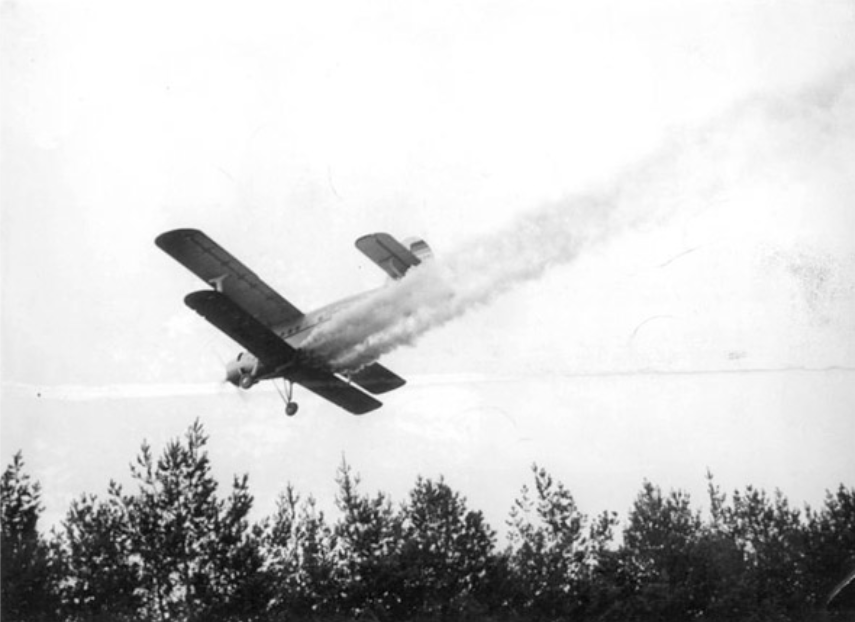
\includegraphics[width=0.75\linewidth]{images/ddt_schaedlingsbekaempfung.png}
\end{center}

\subsection{Katastrophenereignis und schleichende Krise}

Die Vorlesung unterscheidet
zwischen Katastrophenereignissen
und schleichenden Krisen.

Ein Katastrophenereignis ist meist:

\begin{itemize}
\item plötzlich
\item sichtbar
\item lokalisiert
\item datierbar
\item medial gut vermittelbar
\item mit einem Ausnahmezustand verbunden
\end{itemize}

Eine schleichende Krise ist dagegen:

\begin{itemize}
\item prozesshaft
\item häufig unsichtbar
\item diffus
\item global
\item zeitlich entgrenzt
\item schwer einzelnen Verantwortlichen zuzuordnen
\end{itemize}

Diese Unterscheidung hat wichtige Folgen.

Plötzliche Katastrophen erzeugen
mediale Aufmerksamkeit
und politischen Handlungsdruck.

Schleichende Krisen konkurrieren dagegen
mit der Aufmerksamkeitsökonomie.

Sie werfen immer wieder neue Fragen,
Daten
und Zusammenhänge auf.

Dadurch sind sie schwieriger
gesellschaftlich zu bearbeiten.

\subsection{Die Entstehung der Umwelt als gesellschaftspolitisches Problem}

Zwischen 1960 und 1980
wurde „Umwelt“ zunehmend
zu einem gesellschaftspolitischen Problem.

Dabei wirkten mehrere Faktoren zusammen.

Erstens spielten populärwissenschaftliche Bücher
und Medien eine wichtige Rolle.

Die Biologin Rachel Carson veröffentlichte 1962
das Buch \emph{Silent Spring}.

Darin erklärte sie einer breiten Öffentlichkeit
die Auswirkungen von Pestiziden
auf Böden,
Gewässer,
Grundwasser
und Tiere.

In den 1960er und 1970er Jahren
folgten weitere Autorinnen und Autoren.

Wichtige Beispiele sind:

\begin{itemize}
\item \emph{The Population Bomb} von Paul und Anne Ehrlich
\item \emph{The Limits to Growth} des Club of Rome
\item Beiträge des Zukunftsforschers Robert Jungk
\end{itemize}

Diese Texte machten deutlich,
dass Umweltprobleme
nicht isoliert betrachtet werden können.

Sie zeigten den interdependenten Charakter
ökologischer,
technischer
und gesellschaftlicher Systeme.

\subsection{Wissenschaftliche Warnungen und Risikomodelle}

Ein zweiter Faktor war die zunehmende Bedeutung
wissenschaftlicher Warnungen
und Risikomodelle.

Viele Autorinnen und Autoren
populärwissenschaftlicher Umweltliteratur
waren von systemischem
und technokratischem Denken geprägt.

Dieses Denken entwickelte sich
nach dem Zweiten Weltkrieg
besonders im Umfeld von Grossunternehmen,
Militär und Staat.

Wichtige Felder waren:

\begin{itemize}
\item Kybernetik
\item Computermodelle
\item Systemanalyse
\item Operations Research
\end{itemize}

Diese Ansätze versuchten,
Ressourcen,
Lieferketten,
Bevölkerungen
und Kommunikation
als steuerbare Systeme zu verstehen.

Im Verlauf der 1960er und 1970er Jahre
wurde dieses Denken auf ökologische Fragen übertragen.

Dadurch entstanden moderne Umweltwissenschaften.

Umwelt wurde nun als komplexes System verstanden,
in dem menschliches Handeln,
Technik,
Industrie
und Natur miteinander verbunden sind.

\subsection{Katastrophen als Verdichtung komplexer Probleme}

Ein dritter Faktor war die mediale Sichtbarkeit
grosser Katastrophen.

Viele Umweltkatastrophen
wurden nun massenmedial verbreitet
und mit Bildmaterial vermittelt.

Dadurch entstand der Eindruck
einer permanenten
und sich verschärfenden Krise.

Katastrophen wirkten als Verdichtung
komplexer Probleme.

Sie machten sichtbar,
was in schleichenden Umweltkrisen
oft schwer erkennbar blieb:

\begin{itemize}
\item technische Risiken
\item industrielle Verantwortung
\item ökologische Folgen
\item grenzüberschreitende Schäden
\item politische Handlungsnotwendigkeit
\end{itemize}

Ereignisse wie Schweizerhalle,
Tschernobyl,
Bhopal
oder Seveso wurden zu Symbolen
für die Risiken moderner technisierter Gesellschaften.

\subsection{Protestbewegungen und zivile Partizipation}

Ein vierter Faktor war die Entstehung
neuer Protestbewegungen.

Die Erkenntnis,
dass eine technisierte
und auf wirtschaftliches Wachstum ausgerichtete Welt
weitreichende und langfristige Folgen hat,
führte in der Zivilbevölkerung
zu politischem Aktivismus.

Kritisiert wurde unter anderem
der kapitalistische Wachstumsimperativ.

Umweltbewegungen verbanden ökologische Fragen
mit Kritik an Industrie,
Atomenergie,
Konsumgesellschaft
und staatlicher Planung.

Ein wichtiges Beispiel in der Schweiz
war die Besetzung des Baugeländes
des Kernkraftwerks Kaiseraugst im Jahr 1975.

1983 gründete sich die Grüne Partei der Schweiz.

Kurz zuvor hatte sich auch in der Bundesrepublik Deutschland
eine grüne Partei zusammengeschlossen.

\begin{center}
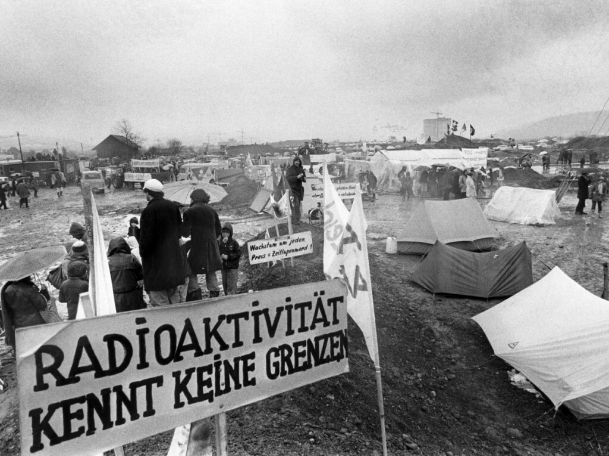
\includegraphics[width=0.75\linewidth]{images/kaiseraugst_1975.png}
\end{center}

\subsection{Politische Verhandlungen}

Ein fünfter Faktor war die politische Bearbeitung
von Umweltfragen.

Einzelne Themen wurden bereits seit den 1950er Jahren
in nationaler und regionaler Politik aufgegriffen.

Dazu gehörten:

\begin{itemize}
\item Langzeitwirkungen atomarer Tests
\item Luftverschmutzung
\item Gewässerschutz
\item gesellschaftliche Leistungen des Waldes
\item Natur- und Artenschutz
\end{itemize}

Zunehmend wurden Umweltfragen
auch international verhandelt.

Ein wichtiger Meilenstein war
die erste Umweltkonferenz in Stockholm 1972.

Dort wurde deutlich,
dass globale Umweltpolitik
unterschiedliche Interessen
miteinander vereinbaren muss.

Vertreterinnen und Vertreter
von Ländern der südlichen Hemisphäre
wehrten sich dagegen,
die gleichen Kosten zu tragen
wie die industrialisierten Länder des Nordens.

Denn diese seien historisch
in viel grösserem Ausmass
für Umweltprobleme verantwortlich.

Auch die Ölkrisen von 1973 und 1979
bildeten einen wichtigen Kontext
für die Umweltdebatte.

\subsection{Umwelt machen}

Die Vorlesung betont,
dass „Umwelt“ nicht einfach
eine natürliche Gegebenheit ist.

Über „Umwelt“ im heutigen Sinn
begann man erst in der zweiten Hälfte
des 20. Jahrhunderts zu sprechen.

Der Begriff existierte zwar bereits seit etwa 1800.

Seine Bedeutung veränderte sich jedoch stark.

Zunächst bedeutete Umwelt
vor allem Umgebung des Menschen.

Später wurde der Begriff
in der Gesellschaftstheorie
als Übersetzung von Milieu verwendet.

Im biologischen Sinn verstand Jakob von Uexküll
unter Umwelt die für ein Lebewesen relevante Umgebung,
die auf seine Lebensbedingungen einwirkt.

Erst um 1970 wurde Umwelt
zum Standardbegriff der ökologischen Bewegung.

Von nun an stand Umwelt
für Natur,
aber auch für Dinge,
Lebewesen,
Vorgänge
und Zusammenhänge,
die in Kontakt und Wechselbeziehung
zum Menschen stehen.

\subsection{Von Natur zu Umwelt}

Vor der modernen Umweltbewegung
sprach man eher von Natur
oder Naturschutz.

Natur wurde dabei häufig
als Gegenbegriff zur Kultur verstanden.

Naturschutz zielte oft auf den Schutz
besonderer Landschaften,
Arten
oder Naturdenkmäler.

Der moderne Umweltbegriff
geht darüber hinaus.

Er beschreibt nicht mehr eine Natur,
die ausserhalb der Gesellschaft steht.

Vielmehr macht er sichtbar,
dass Natur und Kultur
in modernen Gesellschaften
nicht mehr klar voneinander getrennt werden können.

Industrie,
Landwirtschaft,
Chemie,
Verkehr,
Konsum
und Energieversorgung
verändern ökologische Zusammenhänge.

Die zentrale These lautet daher:

Umwelt entsteht historisch dort,
wo die Ununterscheidbarkeit
zwischen Natur und Kultur
in der postmodernen Gesellschaft
sichtbar wird.

\subsection{Historische Antworten auf Umweltprobleme}

Die Vorlesung unterscheidet verschiedene Antworten
auf umweltpolitische Herausforderungen.

Eine erste Antwort ist technische Innovation.

Technologien sollen Probleme lösen,
die selbst technisch oder industriell verursacht wurden.

Produktionsprozesse sollen verbessert,
Schadstoffe reduziert
oder neue Energieformen entwickelt werden.

Diese Strategie kann jedoch
die Komplexität technischer Systeme weiter erhöhen.

Dadurch können neue Abhängigkeiten
und neue Risiken entstehen.

Eine zweite Antwort ist Bevölkerungsregulierung.

Diese ist problematisch,
weil sie zwangsläufig die Frage aufwirft,
wer angeblich „zu viel“ ist.

Historisch zeigt sich dies etwa
an westlich geförderter Geburtenkontrolle
in Indien und China in den 1960er Jahren.

Eine dritte Antwort sind Regulierungen für die Industrie.

Verursacher von Umweltverschmutzung
sollen zur Verantwortung gezogen
und finanziell belastet werden.

Dies ist jedoch schwierig,
weil Industrie politisch gut organisiert ist
und globale Produktions-
und Distributionsprozesse
Verantwortung schwer zuordnen lassen.

Eine vierte Antwort ist die Kommodifizierung von CO2.

Seit den internationalen Klimaverhandlungen
und dem Emissionshandel
werden Umweltprobleme teilweise
in kapitalistische Marktlogiken integriert.

Dadurch wird über Emissionen gehandelt,
anstatt den Wachstumsimperativ selbst
grundsätzlich in Frage zu stellen.

\subsection{Zentrale Erkenntnisse}

Die Vorlesung zeigt,
dass Umweltkatastrophen
und Umweltbewusstsein
eng mit der Geschichte moderner Technik verbunden sind.

Technische Systeme erzeugen nicht nur Fortschritt,
sondern auch Risiken,
Nebenfolgen
und neue Formen politischer Verantwortung.

Zentrale Erkenntnisse sind:

\begin{itemize}
\item Umweltkatastrophen entstehen häufig aus komplexen technischen und organisatorischen Zusammenhängen.
\item In eng gekoppelten Systemen können kleine Störungen zu grossen Krisen eskalieren.
\item Schleichende Umweltkrisen unterscheiden sich stark von plötzlichen Katastrophenereignissen.
\item Umwelt wurde erst im 20. Jahrhundert zu einem zentralen gesellschaftspolitischen Problem.
\item Medien, Wissenschaft, Protestbewegungen und Politik trugen zur Entstehung modernen Umweltbewusstseins bei.
\item Der Begriff Umwelt zeigt, dass Natur und Kultur in modernen Gesellschaften nicht mehr klar trennbar sind.
\item Antworten auf Umweltprobleme bleiben umstritten, weil sie technische, politische, wirtschaftliche und globale Interessen berühren.
\end{itemize}

Die zentrale These lautet:

Umweltprobleme sind keine äusseren Störungen
einer ansonsten funktionierenden technischen Moderne.

Sie sind Teil dieser Moderne selbst.

Die technisierte,
industrialisierte
und wachstumsorientierte Gesellschaft
bringt jene Umweltkrisen hervor,
die sie anschliessend wissenschaftlich,
technisch,
politisch
und gesellschaftlich zu bewältigen versucht.
